\section{Cicli limite, Orbite Periodiche e Wan Der Pol}%
\label{sub:Cicli limite}
\begin{defn}[Ciclo limite]
    Dato un campo vettoriale 
    \[
	\frac{\text{d} \v{x}}{\text{d} t} = F(\v{x}) \quad  \v{x}\in \mathbb{R}^n \quad  F:\mathbb{R}^n\to \mathbb{R}^n
    .\] 
    Un ciclo limite $\gamma$ è una orbita chiusa e \textbf{isolata} tale che $\gamma  \in \omega (\v{x}_p)$ con $\v{x}_p \in \mathbb{R}^n$. 
    \marginpar{
            \captionsetup{type=figure}
            \incfig{4_3_1}
            \caption{\scriptsize }
        \label{fig:4_3_1}
        }
\end{defn}
\noindent
Se si costruisce un intorno di un ciclo limite $N(\gamma)$ si ha che in tale intorno non devono esistere altre orbite periodiche chiuse. Per questo motivo, nello spazio delle fasi il ciclo limite deve essere isolato.\\
\marginpar{
        \captionsetup{type=figure}
        \incfig{4_3_2}
	\caption{\scriptsize Ciclo limite $\gamma$ con il relativo intorno senza orbite periodiche chiuse $N(\gamma) $.}
    \label{fig:4_3_2}
    }

\begin{thm}[Inesistenza dei cicli limite per i sistemi lineari]
Un sistema dinamico lineare $\frac{\text{d} \v{x}}{\text{d} t} = A \v{x}$ non può possedere un ciclo limite.
\end{thm}
\noindent
\begin{proof}
    Si basa sul principio di sovrapposizione. 
    Per casa\ldots
\end{proof}
\begin{defn}[Varietà stabile e instabile locali rispetto a $\gamma$]
    Dato un sistema dinamico con flusso di fase $\varphi_t(\v{x})$, sia $\gamma$ un ciclo limite di tale sistema ed $N$ un suo intorno tale che $N \subset B$ con $B$ bacino di attrazione di $\gamma$.
    \[
	W_{loc}^s(\gamma) = \left\{\v{x}\in N| d(\varphi_t(\v{x}) , \gamma)\to 0 \text{ con } t\to \infty; \ \varphi_t (\v{x}) \in N\right\}
    .\] 
    \[
	W_{loc}^u(\gamma) = \left\{\v{x}\in N| d(\varphi_t(\v{x}) , \gamma)\to 0 \text{ con } t\to -\infty; \ \varphi_t (\v{x}) \in N \right\}
    .\] 
    dove $d(\varphi_t(\v{x}), \gamma)$ è la distanza della varietà dal flusso di fase.
\end{defn}
\noindent
\subsection{Esistenza di Orbite periodiche in $\mathbb{R}^2$}%
\label{sub:Esistenza di Orbite periodiche in} 
Preso un campo vettoriale:
\[
\begin{dcases}
    \frac{\text{d} x}{\text{d} t} = F(x, y) \\
    \frac{\text{d} y}{\text{d} t} = G(x, y) 
\end{dcases}
    \quad  \v{V} = \begin{pmatrix} x \\ y \end{pmatrix} \quad 
    G, F \in C^r \ r\ge 1
\]
\begin{thm}[Criterio di Bendixon]
    Supponiamo che il campo sia definito in $D \subset \mathbb{R}^2$  e che $D$  sia semplicemente connesso.\\
    Se in $D$  la funzione 
    \[
        \frac{\partial F}{\partial x} + \frac{\partial G}{\partial y} 
    .\] 
    Ha sempre lo stesso segno allora in $D$ non può esserci alcuna orbita chiusa.
\end{thm}
\noindent
\begin{proof}
    Prendiamo una superficie $S \subset \mathbb{R}^3$ con contorno $\tau$. Supponiamo di aver definito un campo vettoriale $E$ in $S$.\\
    Facendo una circuitazione lungo $\tau$ di $E$ si può sfruttare il teorema del rotore:
    \[
	\oint_{\tau} \v{E}d\v{s} = \int \int_S (\nabla \times \v{E}) d\v{a}
    .\] 
    Supponiamo di prendere ad esempio il campo:
    \[
	\v{E} = (E_x, E_y, 0)
    .\] 
    E supponiamo la superficie $S$ giacente sul piano $(x, y)$. Allora si ha che $d\v{s} = (dx, dy, 0) $ e $d\v{a} = (0 , 0, dxdy) $.\\
    In questo modo la componente $z$ del rotore di $\v{E}$ è:
    \[
	(\nabla \times \v{E})_z = \frac{\partial E_y}{\partial x} - \frac{\partial E_x}{\partial y} 
    .\] 
    Svolgiamo allora l'integrale:
    \[
        \int_\gamma  \left[E_x dx + E_ydy\right] = \int \int_S \left[\frac{\partial E_y}{\partial x} - \frac{\partial E_x}{\partial y} \right]dxdy
    .\] 
    Poniamo adesso (in riferimento al teorema) $E_x = -G(x, y)$, $E_y = F(x, y) $. Allora si ha che:
    \[
	\int_\gamma  \left[F(x, y) dy - G(x, y) dx\right] = 
	\int \int_S \left[\frac{\partial F}{\partial x} + \frac{\partial G}{\partial y} \right]dxdy
    .\] 
    A questo punto possiamo inserire l'ipotesi del teorema. Supponiamo che la funzione del teorema non sia identicamente nulla e non cambi segno e poniamo $S = D$. Queste due assunzioni portano ad una contraddizione.
    \[
    \begin{dcases}
    \frac{\text{d} x}{\text{d} t} = F\\
    \frac{\text{d} y}{\text{d} t} = G 
    \implies  \frac{\text{d} x}{\text{d} y} = \frac{F}{G}\implies 
    -(dxG-Fdy) = 0
    \end{dcases}
    \]
    E questo contraddice l'espressione che abbiamo ricavato (a sinistra dell'uguale).
\end{proof}
\begin{exmp}[]
    \[
    \begin{dcases}
	\frac{\text{d} x}{\text{d} t} = y = F(x, y) \\
	\frac{\text{d} y}{\text{d} t} = x-x^3-\delta y = G(x, y) 
    \end{dcases}
    \]
    Calcoliamo 
    \[
        \frac{\partial F}{\partial x} + \frac{\partial G}{\partial y} = -\delta
    .\] 
    Quindi l'esisteza di orbite chiuse dipende da $\delta$.
\end{exmp}
\subsection{Oscillatore Wan Der Pole}%
\label{sub:Oscillatore Wan Der Pole}
La particolarità di questo oscillatore è la presenza di un componente elettronico non lineare $V(I)$ tale che:
    \marginpar{
        \captionsetup{type=figure}
        \fbox{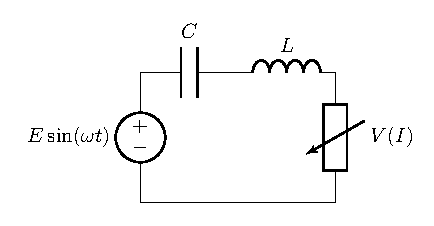
\includegraphics[width=\marginparwidth]{figures/tikz/duffling.pdf}}
        \caption{\scriptsize Schema circuitale dell'oscilaltore di Wan Der Pole}
        \label{fig:tikz-3_rlc-pdf}
    }
\[
    V(I) = RI_0\left[- \frac{I(t) }{I_0} + \frac{1}{3}\left(\frac{I}{I_0}\right)^3\right]
.\] 
L'equazione che regola il circuito è la seguente:
\[
    E\sin (\omega t) = \frac{q}{c}+ L\frac{\text{d} I}{\text{d} t}  + V(I) 
.\] 
Derivando memrbo a membro e ponendo
\[
    \overline{t} = \frac{t}{\sqrt{LC}} \qquad  \mu= \frac{RC}{\sqrt{LC} } \qquad  b = \frac{E C \omega}{I_0}
.\] 
Si ottiene il sistema:
\[
    \frac{\text{d} ^2x}{\text{d} t^2} = -x + \mu \left[1-x^2\right]\frac{\text{d} x}{\text{d} t} + b \cos (\omega t) \quad  t = t'
.\] 
Consideriamo il caso di $b = 0$:
\[
    \frac{\text{d} ^2x}{\text{d} t^2} + \mu\left[x^2-1\right]+x = 0
.\] 
Che costituisce un oscillatore armonico con un attrito per $x > 1$ ed una forza pompante con $x<1$.\\
Vogliamo capire se questo sistema può avere delle orbite periodiche. A tale scopo affrontiamo 3 differenti approcci.
\paragraph{Metodo 1}%
Riportiamo il sistema nella forma canonica:
\[
\begin{dcases}
\frac{\text{d} x}{\text{d} t} = y = F\\
\frac{\text{d} y}{\text{d} t} = -x - m\mu\left[x^2-1\right]y = G
\end{dcases}
\]
Utilizzando il criterio:
\[
    \frac{\partial F}{\partial x} + \frac{\partial G}{\partial y} = - \mu\left[x^2-1\right]
.\] 
Quindi dallo studio del segno di questa quantità si ottengono i due punti annullamento del funzionale: $x=\pm 1$. Se ne deduce che studiando il sistema in regioni nel quale il segno di questa quantità non cambia ($x<-1$  $-1< x < 1$ e $x > 1$) non troveremo orbite periodiche. Tuttavia studiando il sistema in $\mathbb{R}^2$, ad esempio, le orbite periodiche ci potrebbero essere.
\paragraph{Metodo 2: Teorema di Lienard}%
\begin{thm}[Teorema di Lienard]
    Data l'equazione (di Lienard)
    \[
	\frac{\text{d} ^2x}{\text{d} t^2} f(x) \frac{\text{d} x}{\text{d} t} + g(x) = 0
    .\] 
    Supponiamo che $f(x), g(x)$ abbiano le seguenti proprietà:
    \begin{itemize}
	\item $f(x) , g(x) \in C^r$ con $r\ge 1$.
	\item $f(x) = f(-x)$ (pari).
	\item $g(x) = -g(-x)$ (dispari).
	\item $g(x) >0 $ per $x > 0$.
	\item Si definisce la funzione integrale:
	    \[
		\int_{0}^{x} f(s) ds = F(x)
	    .\] 
	    E si deve verificare che 
	    \begin{itemize}
		\item $\exists x > 0$ tale che $F(c) =0$.
		\item $F(x) < 0$ con $0<x<c$.
		\item $F(x) >0 $ per $x> 0$ e $F(x)$ non decrescente ed inoltre:
		    \[
			\lim_{x \to \infty} f(x) = \infty
		    .\] 
	    \end{itemize}
    \end{itemize}
    Allora esiste un ciclo limite intorno all'origine.
\end{thm}
\noindent
Applichiamo il teorema all'oscillatore Van Der Pole.
\[
    \frac{\text{d} ^2x}{\text{d} t^2} + \mu\left(x^2-1\right)\frac{\text{d} x}{\text{d} t} + x = 0 \quad  \mu  > 0
.\] 
Si ha che 
\[
    f(x) = \mu(x^2-1) \qquad  g(x) = x
.\] 
Tutte le condizioni sono rispettate banalmente, l'unica più complicata è l'ultima:
\[
    F(x) = \int_{0}^{x} \mu (s^2-1) ds = \mu x\left[\frac{x^2}{3}-1\right] 
.\] 
Si trova che serve $c = \sqrt{3} $, è vero che $F(x) < 0$  se $0<x<\sqrt{3}$  ed anche la condizione $F(x) >0$  per $x >\sqrt{3}$. La condizione di limite è anch'essa rispettata per cui vale la tesi.
\paragraph{Metodo 3: Phase Portrait.}%
\begin{defn}[Nurk Lines]
    Prendiamo un sistema dinamico:
    \[
    \begin{dcases}
	\frac{\text{d} x}{\text{d} t} = F(x, y) \\
	\frac{\text{d} y}{\text{d} t} = G(x, y) 
    \end{dcases}
    \]
    Si definiscono Nurk Lines gli insiemi:
    \[\begin{aligned}
	& N_x = \left\{(x, y) \in \mathbb{R}^2 | F(x, y) = 0\right\}\\
	& N_y = \left\{(x, y) \in \mathbb{R}^2 | G(x, y) = 0\right\}
    .\end{aligned}\]
    Le cui intersezioni sono i punti stazionari.
\end{defn}
\noindent
Riprendiamo allora l'oscillatore:
\[
    \frac{\text{d} ^2x}{\text{d} t^2} + \mu\left(x^2-1\right)\frac{\text{d} x}{\text{d} t} + x = 0 \quad  \mu  > 0
.\] 
Questa volta non si utilizza il sistema canonico ma definiamo la $y$ come:
\[
    y = x-\frac{x^3}{3} - \frac{1}{\mu}\frac{\text{d} x}{\text{d} t} 
.\] 
in questo modo derivando otteniamo:
\[
    \frac{\text{d} y}{\text{d} t} = -\frac{1}{\mu}\left[-\frac{\text{d} ^2x}{\text{d} t^2} - \mu (x^2-1) \frac{\text{d} x}{\text{d} t} \right] = \frac{x}{\mu}
.\] 
Per la variabile $x$  invece si ottiene (invertendo la relazione per $y$):
\marginpar{
        \captionsetup{type=figure}
        \incfig{4_3_3}
        \caption{\scriptsize Andamento delle Nurk lines ed una possibile orbita periodica}
    \label{fig:4_3_3}
    }
\[
    \frac{\text{d} x}{\text{d} t} = \mu\left[x-\frac{x^3}{3}-y\right]
.\] 
Utilizzando queste due equazioni possiamo determinare gli stati stazioari e la loro stabilità (per casa). Utilizzando le nurk lines si ha che:
\[\begin{aligned}
    &N_x = \left\{(x, y) \in \mathbb{R}^2| y = x-\frac{x^3}{3}\right\}\\
    &N_y = \left\{(x, y) \in \mathbb{R}^2| x = 0\right\}
.\end{aligned}\]
Queste regioni indicano il cambio di segno del campo vettoriale $\frac{\text{d} \v{x}}{\text{d} t}$.\\
Nella figura \ref{fig:4_3_3} sono rappresentate le Nurk lines per il caso in questione. Si nota che la regione delimitata dalla linea gialla è una regione di intrappolamento (le linee di livello puntano sempre verso l'interno di tale regione. Come conseguenza questa è una regione positivamente invariante (compatta), quindi ogni $\begin{pmatrix} x \\ y \end{pmatrix}$ in tale regione cadrà su una orbita periodica in quanto il punto stazionario nell'origine è un punto stabile (ed è l'unico).
